\documentclass[12pt,letterpaper]{article}
\usepackage[utf8]{inputenc}
\usepackage[spanish]{babel}
\usepackage{graphicx}
\usepackage[left=2cm,right=2cm,top=2cm,bottom=2cm]{geometry}
\usepackage{graphicx} % figuras
\usepackage{hyperref}
% \usepackage{subfigure} % subfiguras
\usepackage{float} % para usar [H]
\usepackage{amsmath}
%\usepackage{txfonts}
\usepackage{stackrel} 
\usepackage{multirow}
\usepackage{enumerate} % enumerados
\renewcommand{\labelitemi}{$-$}
\renewcommand{\labelitemii}{$\cdot$}
% \author{}
% \title{Caratula}
\begin{document}

% Fancy Header and Footer
% \usepackage{fancyhdr}
% \pagestyle{fancy}
% \cfoot{}
% \rfoot{\thepage}
%

% \usepackage[hidelinks]{hyperref} % CREA HYPERVINCULOS EN INDICE

% \author{}
\title{Caratula}

\begin{titlepage}
\begin{center}
\large{UNIVERSIDAD PRIVADA-DE-TACNA}\\
\vspace*{-0.025in}
\begin{figure}[htb]
\begin{center}

\includegraphics[width=8cm]{./Imagenes/logo}
\end{center}
\end{figure}
\vspace*{0.15in}
INGENIERIA DE SISTEMAS  \\

\vspace*{0.5in}
\begin{large}
TITULO:\\
\end{large}

\vspace*{0.1in}
\begin{Large}
\textbf{INFORME DE LABORATORIO No 02} \\
\end{Large}

\vspace*{0.3in}
\begin{Large}
\textbf{CURSO:} \\
\end{Large}

\vspace*{0.1in}
\begin{large}
INTELIGENCIA DE NEGOCIOS\\
\end{large}

\vspace*{0.3in}
\begin{Large}
\textbf{DOCENTE(ING):} \\
\end{Large}

\vspace*{0.1in}
\begin{large}
 Patrick Cuadros Quiroga\\
\end{large}

\vspace*{0.2in}
\vspace*{0.1in}
\begin{large}
Integrante: \\
\begin{flushleft}
Nilson Felix Laura Atencio	\hfill	(2015053846) 
\end{flushleft}
\end{large}
\end{center}

\end{titlepage}



\thispagestyle{empty} % INDICE SIN NUMERO
\newpage
\setcounter{page}{1} % REINICIAR CONTADOR DE PAGINAS DESPUES DEL INDICE


\section{DESARROLLO}
\subsection{Crear relaciones}
\begin{itemize}
	\item \textbf{Tarea 1:} Relaciones autómaticas
	\item Iniciar Power Bi Desktop; click en Obtener Datos , click en EXCEL y luego click en Conectar.
	\item En el cuadro de dialogo Abrir, buscar el archivo Adventure Works Sales Data.xlsx, y hacer
click en Abrir. 
	\item En el cuadro de dialogo Explorador, seleccionar las hojas DimCurrency, DimCustomer,
DimDate, DimProduct, DimPromotion, DimSalesTerritory, y FactInternetSales, y luego hacer click en Cargar.

	\item En el panel de vistas a mano derecho, hacer click en Relaciones, hacer click en Administrar relaciones.
\begin{center}
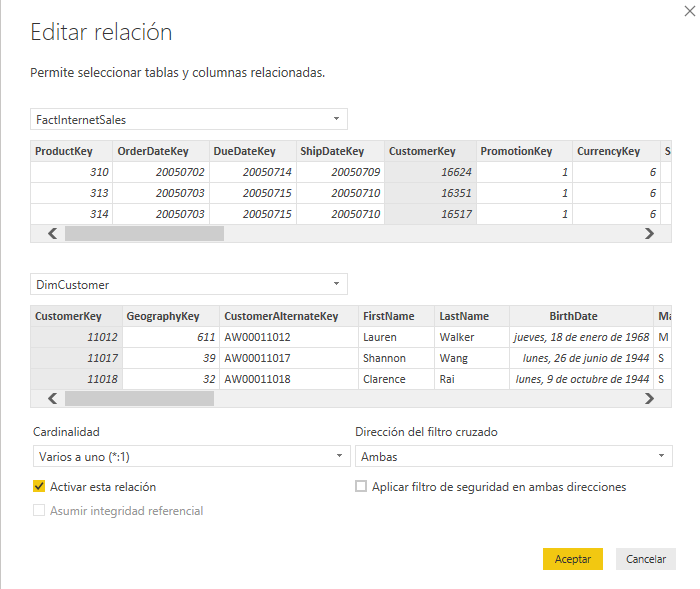
\includegraphics[width=12cm]{./Imagenes/2-}
\end{center}
	\item \textbf{Tarea 2:} Relaciones manuales
	\item En la Ventana de Power BI Desktop, click en Obtener Datos y luego en Excel, abrir el archivo Adventure Works Product Categories.xlsx.
	\item En el cuadro de dialogo Explorador, seleccionar las hojas DimProductCategory, and
DimProductSubcategory, y luego hacer click en Cargar.
\begin{center}
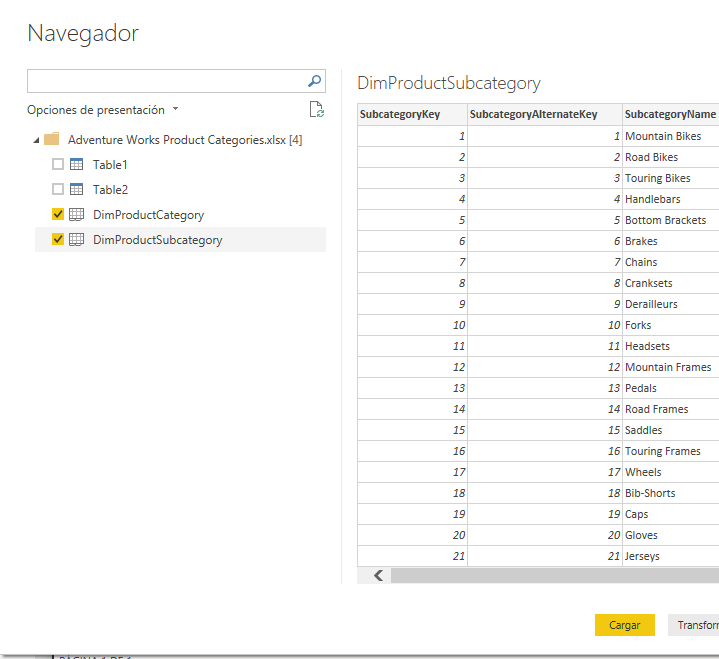
\includegraphics[width=12cm]{./Imagenes/3}
\end{center}
\begin{center}
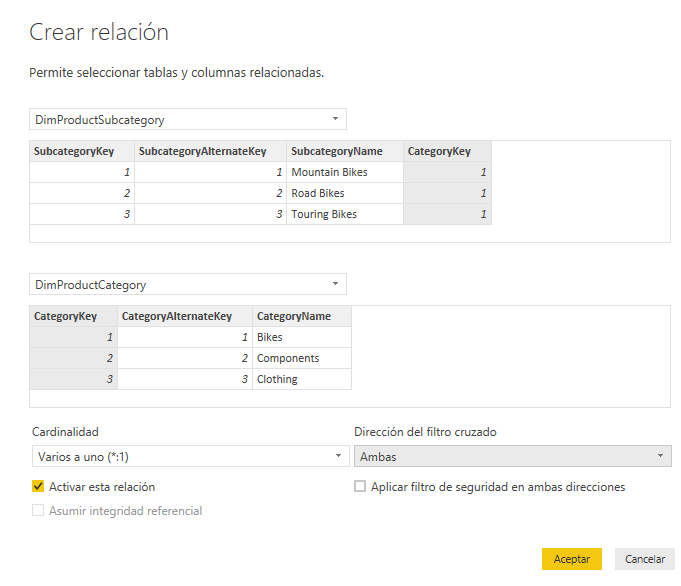
\includegraphics[width=12cm]{./Imagenes/4}
\end{center}
\end{itemize}
\subsection{Cálculos}
\begin{itemize}
	\item En Power Bi Desktop, en el panel del lado izquierdo, clic en Datos.
	\item En el panel de Modelado, en el grupo de calculaciones, clic en Nueva Columna.
\begin{center}
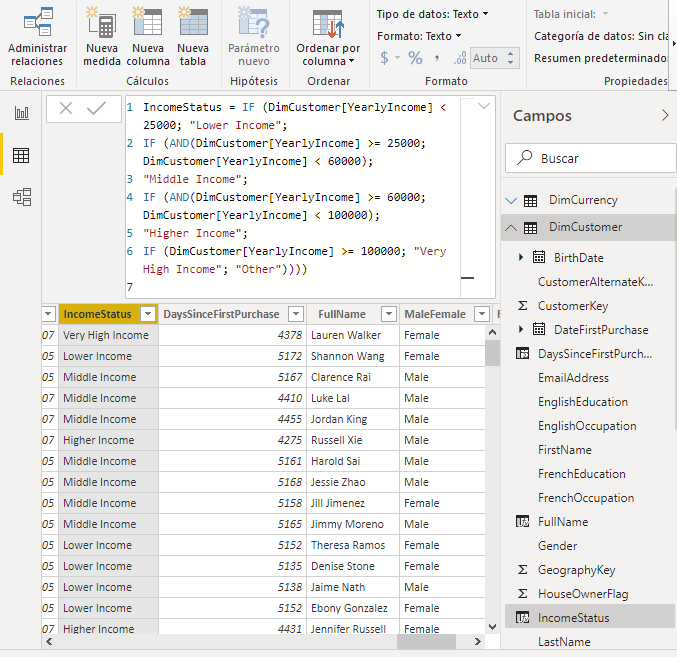
\includegraphics[width=12cm]{./Imagenes/5}
\end{center}
\begin{center}
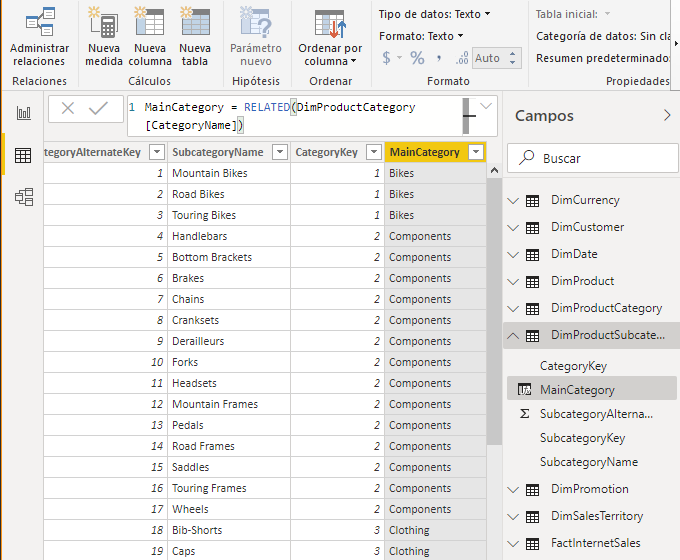
\includegraphics[width=12cm]{./Imagenes/6}
\end{center}
\begin{center}
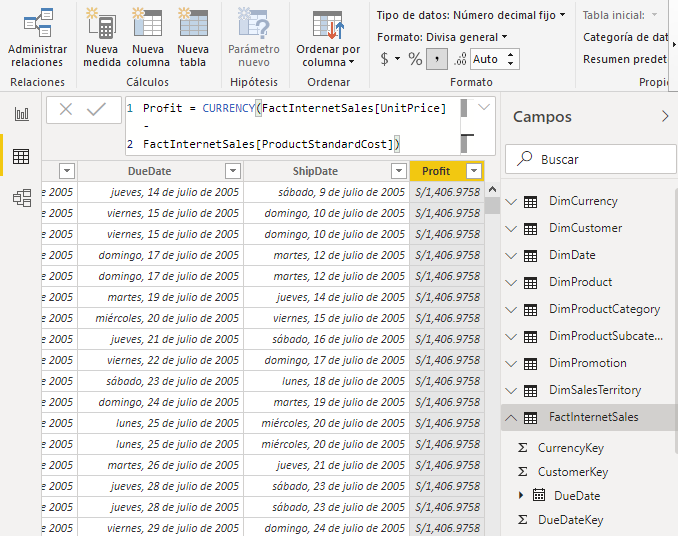
\includegraphics[width=12cm]{./Imagenes/8}
\end{center}

\end{itemize}

\end{document}
